%% ============================================================
%% AlgoProfessor AI Scientist — Hands-On Syllabus (Sunday Edition)
%% 6 Sundays x 5 hours = 30 hours | 2 h teaching + 3 h real-time work
%% Compile: pdflatex (run twice)
%% ============================================================
\documentclass[11pt,a4paper]{article}

\usepackage[T1]{fontenc}
\usepackage[utf8]{inputenc}
\usepackage{mathptmx}  % Times (New Roman) for text and maths
\usepackage{pgfplots}
\pgfplotsset{compat=1.17}
\usepackage{caption}
\usepackage{pdflscape}
\usepackage{microtype}
\usepackage[a4paper,margin=1.8cm,top=2.2cm,bottom=2.2cm,headheight=15pt]{geometry}
\usepackage[table]{xcolor}
\usepackage{tikz}
\usetikzlibrary{positioning,shapes,arrows.meta,calc,decorations.pathreplacing}
\usepackage[most]{tcolorbox}
\usepackage{tabularx,booktabs,array,multirow}
\usepackage{enumitem}
\usepackage{titlesec}
\usepackage{fancyhdr}
\usepackage{lastpage}
\usepackage[hidelinks]{hyperref}

%% ---------------- Colour code ----------------
\definecolor{navy}{HTML}{0B1F3A}
\definecolor{navylight}{HTML}{1F3B63}
\definecolor{gold}{HTML}{C9A227}
\definecolor{goldlight}{HTML}{F6EBC4}
\definecolor{paper}{HTML}{FBF8EF}
\definecolor{ink}{HTML}{1A1A1A}
\definecolor{saffron}{HTML}{FF9933}
\definecolor{indgreen}{HTML}{138808}
% Mode colours
\definecolor{teach}{HTML}{C9A227}   % Gold  = Hands-on teaching
\definecolor{work}{HTML}{0B1F3A}    % Navy  = Real-time work
\definecolor{dataC}{HTML}{1E7B5A}   % Green = Dataset
\definecolor{skillC}{HTML}{6A3D9A}  % Purple= Skill set
% Sunday theme colours
\definecolor{sunA}{HTML}{0F6E7A} % S1 Teal      - Data & ML
\definecolor{sunB}{HTML}{A4243B} % S2 Ruby      - Deep Learning
\definecolor{sunC}{HTML}{5B3A8E} % S3 Violet    - Transformers & LLMs
\definecolor{sunD}{HTML}{2E7D32} % S4 Emerald   - RAG
\definecolor{sunE}{HTML}{C25E00} % S5 Amber     - Agentic AI
\definecolor{sunF}{HTML}{1F4E9C} % S6 Royal     - Production & Capstone

\color{ink}
\renewcommand{\familydefault}{\rmdefault}
% Times New Roman only: map sans and mono families to Times as well
\renewcommand{\sfdefault}{\rmdefault}
\renewcommand{\ttdefault}{\rmdefault}
\captionsetup[figure]{font=small,labelfont={bf,color=navy},textfont={color=navylight},labelsep=period,skip=4pt}
\setlength{\parindent}{0pt}
\setlength{\parskip}{4pt}

%% ---------------- Headings ----------------
\titleformat{\section}{\sffamily\Large\bfseries\color{navy}}{\thesection}{0.6em}{}[{\color{gold}\titlerule[1.2pt]}]
\titleformat{\subsection}{\sffamily\large\bfseries\color{navylight}}{\thesubsection}{0.5em}{}
\titlespacing*{\section}{0pt}{14pt}{8pt}

%% ---------------- Header / footer ----------------
\pagestyle{fancy}
\fancyhf{}
\renewcommand{\headrulewidth}{0pt}
\fancyhead[L]{\sffamily\footnotesize\color{navy}\textbf{AlgoProfessor} AI Scientist --- Hands-On Syllabus}
\fancyhead[R]{\sffamily\footnotesize\color{gold}Sunday Edition $\cdot$ 30 Hours}
\fancyfoot[L]{\sffamily\scriptsize\color{navylight}www.algoprofessor.com $\cdot$ ceo@algoprofessor.com}
\fancyfoot[R]{\sffamily\scriptsize\color{navylight}Page \thepage\ of \pageref{LastPage}}
\fancyfoot[C]{\tikz{\fill[gold](0,0) rectangle (3,0.04);}}

%% ---------------- Helpers ----------------
\newcommand{\teachtag}{\tikz[baseline=(t.base)]\node[fill=teach,text=navy,rounded corners=2pt,inner sep=2pt,font=\sffamily\scriptsize\bfseries](t){TEACH};}
\newcommand{\worktag}{\tikz[baseline=(t.base)]\node[fill=work,text=gold,rounded corners=2pt,inner sep=2pt,font=\sffamily\scriptsize\bfseries](t){BUILD};}
\newcommand{\ds}[1]{{\color{dataC}\bfseries #1}}
\newcommand{\sk}[1]{{\color{skillC}#1}}
\newcolumntype{L}[1]{>{\raggedright\arraybackslash}p{#1}}
\newcolumntype{Y}{>{\raggedright\arraybackslash}X}
\renewcommand{\arraystretch}{1.35}

\newtcolorbox{sundaybox}[3]{enhanced,colback=white,colframe=#1,
  boxrule=0.9pt,arc=3pt,left=6pt,right=6pt,top=6pt,bottom=6pt,
  title={\sffamily\bfseries\large #2\quad\normalsize\color{gold}$\cdot$\quad #3},
  coltitle=white,colbacktitle=#1,attach boxed title to top left={yshift=-1mm},
  boxed title style={sharp corners,boxrule=0pt},fonttitle=\sffamily}

\newtcolorbox{goldnote}[1][]{enhanced,colback=goldlight,colframe=gold,boxrule=0.6pt,arc=2pt,
  left=6pt,right=6pt,top=4pt,bottom=4pt,fontupper=\small,#1}
\newtcolorbox{navynote}[1][]{enhanced,colback=navy,colframe=gold,boxrule=0.8pt,arc=2pt,
  left=8pt,right=8pt,top=6pt,bottom=6pt,coltext=white,fontupper=\small,#1}

\setlist[itemize]{leftmargin=1.2em,itemsep=1pt,topsep=2pt}

%% Sunday hour table
\newenvironment{hourtable}[1]{%
  \small
  \rowcolors{2}{#1!6}{white}
  \tabularx{\linewidth}{@{}>{\centering\arraybackslash}p{0.55cm} >{\centering\arraybackslash}p{1.15cm} Y L{3.5cm} L{3.6cm}@{}}
  \rowcolor{#1}\color{white}\sffamily\bfseries Hr & \color{white}\sffamily\bfseries Mode &
  \color{white}\sffamily\bfseries Topic \& Hands-on Activity &
  \color{white}\sffamily\bfseries Dataset &
  \color{white}\sffamily\bfseries Skill Set Gained\\
}{\endtabularx}

\begin{document}

%% ======================= COVER =======================
\thispagestyle{empty}

\begin{tikzpicture}[remember picture,overlay]
  \fill[white] (current page.north west) rectangle (current page.south east);
  %% tricolour bands (saffron top, green bottom)
  \fill[saffron] (current page.north west) rectangle ($(current page.north east)+(0,-1.1)$);
  \fill[white]   ($(current page.north west)+(0,-1.1)$) rectangle ($(current page.north east)+(0,-1.5)$);
  \fill[indgreen] ($(current page.south west)+(0,1.1)$) rectangle (current page.south east);
  \fill[gold] ($(current page.north west)+(0,-1.5)$) rectangle ($(current page.north east)+(0,-1.6)$);
  \fill[gold] ($(current page.south west)+(0,1.1)$) rectangle ($(current page.south east)+(0,1.2)$);
  %% soft tricolour side ribbon
  \fill[saffron!12] ($(current page.north east)+(-4.2,-1.6)$) rectangle ($(current page.north east)+(-2.8,-27.5)$);
  \fill[white]      ($(current page.north east)+(-2.8,-1.6)$) rectangle ($(current page.north east)+(-1.4,-27.5)$);
  \fill[indgreen!12]($(current page.north east)+(-1.4,-1.6)$) rectangle ($(current page.north east)+(0,-27.5)$);
  \node[anchor=north west,text=navy,font=\sffamily\bfseries\Large] at ($(current page.north west)+(2,-2.4)$) {AlgoProfessor};
  \node[anchor=north west,text=navylight,font=\sffamily\small] at ($(current page.north west)+(2,-3.2)$) {AI R\&D Solutions $\cdot$ Hyderabad, India};
  \node[anchor=north west,text=saffron,font=\sffamily\bfseries\small] at ($(current page.north west)+(2,-5.6)$) {MADE IN INDIA \;$\cdot$\; TRAINING FOR THE WORLD};
  \node[anchor=north west,text=navy,font=\sffamily\bfseries\fontsize{40}{44}\selectfont,align=left] at ($(current page.north west)+(2,-6.4)$) {AI Scientist};
  \node[anchor=north west,text=gold!85!black,font=\sffamily\bfseries\fontsize{22}{26}\selectfont,align=left] at ($(current page.north west)+(2,-8.4)$) {Hands-On Syllabus};
  \node[anchor=north west,text=ink,font=\sffamily\large,align=left,text width=14.5cm] at ($(current page.north west)+(2,-10.0)$)
   {Sunday Edition $\cdot$ 6 Sundays $\cdot$ 30 Hours\\[3pt]
    \color{indgreen}2 hours hands-on teaching \;+\; 3 hours real-time project work, every Sunday};
  %% stat tiles
  \foreach \x/\n/\l/\c in {0/30/Contact hours/saffron,1/18/Real-time build hours/navy,2/30/Datasets (one per hour)/indgreen,3/90+/Skills gained/gold}{
    \node[draw=\c,line width=1pt,fill=\c!8,text=navy,minimum width=3.3cm,text width=3.0cm,minimum height=2.1cm,align=center,
          font=\sffamily,anchor=north west] at ($(current page.north west)+(2+\x*3.6,-13.0)$)
          {{\color{\c!85!black}\fontsize{24}{26}\selectfont\bfseries \n}\\[2pt]\small \l};
  }
  %% fee panel
  \node[anchor=north west,fill=navy,text=white,rounded corners=3pt,inner sep=8pt,text width=14.0cm,align=left,font=\sffamily]
    at ($(current page.north west)+(2,-16.0)$)
    {{\color{gold}\bfseries Programme fee}\\[3pt]
     {\large\bfseries INR 50,000} \;{\small(Hyderabad \& Shirdi, India)}\qquad
     {\large\bfseries US\$ 1,000} \;{\small(USA \& Canada)}};
  \node[anchor=north west,text=navy,font=\sffamily,align=left,text width=14cm] at ($(current page.north west)+(2,-18.6)$)
   {\textbf{\color{saffron}Offline campuses}\\[2pt]
    Hyderabad (India) \quad$\cdot$\quad Shirdi (India) \quad$\cdot$\quad USA \quad$\cdot$\quad Canada};
  \node[anchor=north west,text=navy,font=\sffamily,align=left,text width=14cm] at ($(current page.north west)+(2,-20.4)$)
   {\textbf{\color{indgreen}Career focus}\\[2pt] 16 job roles at top AI companies, global capability centres and AI start-ups\\
    Skills mapped from 2026 to 2035};
  \node[anchor=south west,text=navy,font=\sffamily\small,align=left,text width=14cm] at ($(current page.south west)+(2,1.7)$)
   {\textbf{\color{saffron}Course Director:} Dr S Satyanarayana Ph.D., PDF(AI), FARSC\\
    Founder, CEO \& Chief Agentic AI Scientist $\cdot$ AlgoProfessor AI R\&D Solutions, Hyderabad\\
    Creator of AlgoLang};
  \node[anchor=south,text=white,font=\sffamily\scriptsize] at ($(current page.south)+(0,0.4)$) {www.algoprofessor.com \;$\cdot$\; ceo@algoprofessor.com};
\end{tikzpicture}
\null\newpage

%% ======================= 1. OVERVIEW =======================
\section{Course at a Glance}

\begin{tabularx}{\linewidth}{@{}>{\sffamily\bfseries\leavevmode\color{navy}}L{3.4cm} Y@{}}
\toprule
Programme & AlgoProfessor AI Scientist --- Hands-On (Level 1), Sunday Edition\\
Format & Offline, classroom + lab. Sundays only.\\
Duration & 6 consecutive Sundays $\times$ 5 hours = \textbf{30 contact hours}\\
Weekly split & \teachtag\ 2 hours hands-on teaching \quad + \quad \worktag\ 3 hours real-time project work\\
Campuses & Hyderabad $\cdot$ Shirdi $\cdot$ USA $\cdot$ Canada (venue confirmed on enrolment)\\
Batch size & Maximum 30 learners per campus, 1 mentor per 10 learners in BUILD hours\\
Who it is for & Final-year B.Tech/M.Tech/MCA/M.Sc students, working engineers moving into AI, researchers and founders\\
Outcome & 6 GitHub portfolio projects, 1 deployed capstone, a Demo Day pitch and a mock-interview report\\
Programme fee & \textbf{INR 50,000} per learner (Hyderabad, Shirdi) \quad$\cdot$\quad \textbf{US\$ 1,000} per learner (USA, Canada)\\
Fee includes & All 30 hours, lab mentoring, cloud GPU lab credits for course work, Demo Day, mock interview, certificate\\
Certificate & \emph{AlgoProfessor Certified AI Scientist --- Hands-On (Level 1)}\\
\bottomrule
\end{tabularx}

\subsection*{Colour code used in this syllabus}
\begin{tabularx}{\linewidth}{@{}l Y l Y@{}}
\teachtag & Hands-on teaching hour (instructor-led, live coding) & \worktag & Real-time work hour (team build, mentor review)\\
\ds{Green} & Dataset used in that hour & \sk{Purple} & Skill set gained in that hour\\
\end{tabularx}

\vspace{4pt}
\begin{center}
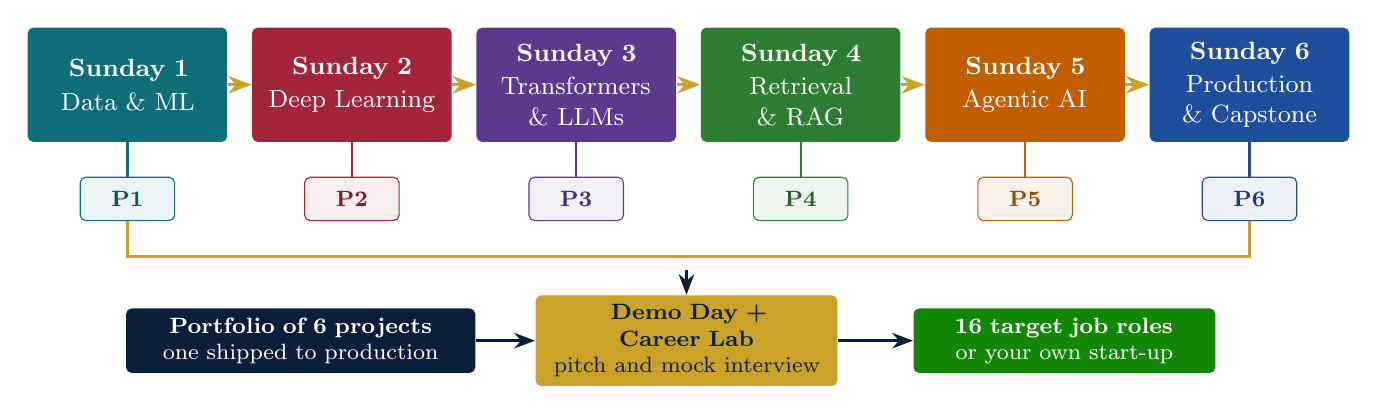
\begin{tikzpicture}[x=1cm,y=1cm,font=\footnotesize]
  \foreach \i/\c/\t/\s/\pp in {0/sunA/Data \& ML/Sunday 1/P1,1/sunB/Deep Learning/Sunday 2/P2,2/sunC/Transformers \& LLMs/Sunday 3/P3,
                           3/sunD/Retrieval \& RAG/Sunday 4/P4,4/sunE/Agentic AI/Sunday 5/P5,5/sunF/Production \& Capstone/Sunday 6/P6}{
    \node[fill=\c,text=white,text width=2.3cm,minimum height=1.45cm,align=center,rounded corners=2pt,font=\small]
      (n\i) at (\i*2.85,0) {\textbf{\s}\\[1pt]\t};
    \node[draw=\c,fill=\c!8,text=\c!80!black,minimum width=1.2cm,minimum height=0.55cm,rounded corners=2pt,font=\footnotesize\bfseries]
      (p\i) at (\i*2.85,-1.45) {\pp};
    \draw[\c,line width=0.8pt] (n\i.south) -- (p\i.north);
  }
  \foreach \i [evaluate=\i as \j using int(\i+1)] in {0,...,4}{\draw[-{Stealth},gold,line width=1.2pt] (n\i.east) -- (n\j.west);}
  \draw[gold,line width=1pt] (p0.south) -- ++(0,-0.45) -| (p5.south);
  \node[fill=navy,text=white,rounded corners=2pt,minimum height=0.75cm,text width=4.2cm,align=center] (cap) at (2.2,-3.25)
     {\textbf{Portfolio of 6 projects}\\ one shipped to production};
  \node[fill=gold,text=navy,rounded corners=2pt,minimum height=0.75cm,text width=3.6cm,align=center] (dd) at (7.1,-3.25)
     {\textbf{Demo Day + Career Lab}\\ pitch and mock interview};
  \node[fill=indgreen,text=white,rounded corners=2pt,minimum height=0.75cm,text width=3.6cm,align=center] (job) at (11.9,-3.25)
     {\textbf{16 target job roles}\\ or your own start-up};
  \draw[-{Stealth},navy,line width=1pt] (7.1,-2.35) -- (dd.north);
  \draw[-{Stealth},navy,line width=1pt] (cap) -- (dd);
  \draw[-{Stealth},navy,line width=1pt] (dd) -- (job);
\end{tikzpicture}
\captionof{figure}{Programme architecture. Each Sunday ends in one portfolio project (P1--P6); together they lead to Demo Day and the job market.}
\end{center}

\newpage
\begin{center}
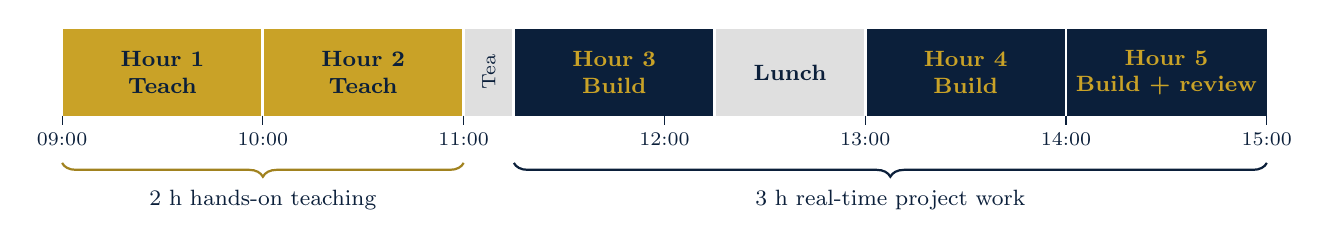
\begin{tikzpicture}[x=2.55cm,y=1cm,font=\footnotesize]
  \foreach \a/\b/\c/\t in {0/1/teach/Hour 1\\Teach,1/2/teach/Hour 2\\Teach,2/2.25/gray!25/,2.25/3.25/work/Hour 3\\Build,
                          3.25/4/gray!25/Lunch,4/5/work/Hour 4\\Build,5/6/work/Hour 5\\Build + review}{
    \fill[\c] (\a,0) rectangle (\b,1.1);
    \draw[white,line width=1pt] (\a,0) -- (\a,1.1);
  }
  \foreach \a/\b/\t/\col in {0/1/Hour 1\\Teach/navy,1/2/Hour 2\\Teach/navy,2.25/3.25/Hour 3\\Build/gold,
                          3.25/4/Lunch/navy,4/5/Hour 4\\Build/gold,5/6/Hour 5\\Build + review/gold}{
    \node[align=center,text=\col,font=\footnotesize\bfseries] at ({(\a+\b)/2},0.55) {\t};
  }
  \node[rotate=90,font=\scriptsize,text=navy] at (2.125,0.55) {Tea};
  \foreach \x/\l in {0/09:00,1/10:00,2/11:00,3/12:00,4/13:00,5/14:00,6/15:00}{
    \draw[navy] (\x,0) -- (\x,-0.12); \node[below,font=\scriptsize,text=navy] at (\x,-0.1) {\l};
  }
  \draw[decorate,decoration={brace,amplitude=5pt,mirror},gold!80!black,line width=0.8pt] (0,-0.6) -- (2,-0.6)
     node[midway,below=6pt,font=\footnotesize,text=navy]{2 h hands-on teaching};
  \draw[decorate,decoration={brace,amplitude=5pt,mirror},navy,line width=0.8pt] (2.25,-0.6) -- (6,-0.6)
     node[midway,below=6pt,font=\footnotesize,text=navy]{3 h real-time project work};
\end{tikzpicture}
\captionof{figure}{The same 5-hour structure runs every Sunday at every campus (local time).}
\end{center}

\subsection*{Standard Sunday timetable (local time at every campus)}
\begin{tabularx}{\linewidth}{@{}L{3.0cm} c Y@{}}
\toprule
\sffamily\bfseries Time & \sffamily\bfseries Mode & \sffamily\bfseries Block\\
\midrule
09:00 -- 10:00 & \teachtag & Hour 1 --- concept + live coding\\
10:00 -- 11:00 & \teachtag & Hour 2 --- concept + live coding\\
11:00 -- 11:15 & --- & Tea break\\
11:15 -- 12:15 & \worktag & Hour 3 --- real-time build sprint 1\\
12:15 -- 13:00 & --- & Lunch\\
13:00 -- 14:00 & \worktag & Hour 4 --- real-time build sprint 2\\
14:00 -- 15:00 & \worktag & Hour 5 --- build sprint 3, demo and mentor review\\
\rowcolor{saffron!15}\textbf{by 18:00} & \textbf{GIT} & \textbf{Mandatory GitHub submission} of the day's project (tagged release + submission form)\\
\bottomrule
\end{tabularx}

\subsection*{Prerequisites and setup (before Sunday 1)}
\begin{itemize}
  \item Python basics (loops, functions, lists, dictionaries). A 4-hour pre-course primer is sent on enrolment.
  \item Laptop with 16 GB RAM recommended. GPU work runs on Google Colab, Kaggle Notebooks or cloud credits.
  \item Accounts: GitHub, Hugging Face, Kaggle. A free LLM API key or a local Ollama install.
  \item Tool stack: Python 3.11+, VS Code, Jupyter, Git, Docker Desktop.
\end{itemize}

%% ======================= 2. SUNDAYS =======================
\newpage
\section{Hour-by-Hour Syllabus}

%% ---------- SUNDAY 1 ----------
\begin{sundaybox}{sunA}{Sunday 1 --- Data \& Machine Learning Foundations}{Hours 1--5}
\textbf{Goal:} think like a data scientist. Frame a business problem, clean data, build and explain a model, track experiments.\par\smallskip
\begin{hourtable}{sunA}
1 & \teachtag & Scientific Python: NumPy vectorisation, Pandas, exploratory data analysis, missing values, outliers, visual EDA. &
  \ds{UCI Adult Income} (48,842 rows, 14 features) & \sk{NumPy, Pandas, Matplotlib/Seaborn, data cleaning, EDA reasoning}\\
2 & \teachtag & Supervised ML pipeline: train/validation/test, cross-validation, regression and classification metrics, gradient boosting. &
  \ds{California Housing} (20,640 districts; scikit-learn) & \sk{scikit-learn Pipelines, k-fold CV, XGBoost/LightGBM, feature engineering}\\
3 & \worktag & Live project kick-off: customer churn. Frame the business question, define the success metric, build a baseline. &
  \ds{IBM Telco Customer Churn} (7,043 customers) & \sk{Problem framing, baseline thinking, metric selection (F1, ROC-AUC)}\\
4 & \worktag & Improve the model: class imbalance, Optuna hyperparameter search, SHAP explanations for business users. &
  \ds{IBM Telco Customer Churn} & \sk{Optuna, class weighting/SMOTE, SHAP explainability}\\
5 & \worktag & Track experiments in MLflow, publish the repo, 3-minute stakeholder presentation, mentor review. &
  \ds{Telco + own MLflow runs} & \sk{MLflow, Git/GitHub workflow, technical storytelling}\\
\end{hourtable}
\begin{goldnote}\textbf{Deliverable P1:} \emph{Churn Intelligence} --- GitHub repo with notebook, MLflow logs, SHAP report and a one-page business summary.\\[2pt]{\color{saffron!80!black}\bfseries GitHub deadline: 18:00 local time, Sunday 1} --- push, tag \texttt{sunday-1}, submit the release link.\end{goldnote}
\end{sundaybox}

\vspace{6pt}
%\newpage
% ---------- SUNDAY 2 ----------
\begin{sundaybox}{sunB}{Sunday 2 --- Deep Learning with PyTorch}{Hours 6--10}
\textbf{Goal:} write training loops yourself, use transfer learning well, and ship an image model that runs on a phone.\par\smallskip
\begin{hourtable}{sunB}
6 & \teachtag & Tensors, autograd, the training loop from scratch, MLPs, optimisers (SGD, Adam), regularisation. &
  \ds{Fashion-MNIST} (70,000 images, 10 classes) & \sk{PyTorch core, autograd, custom training loops, debugging loss curves}\\
7 & \teachtag & CNNs, data augmentation, transfer learning with ResNet/EfficientNet, GPU and mixed precision. &
  \ds{CIFAR-10} (60,000 images) & \sk{CNN design, transfer learning, augmentation, AMP training}\\
8 & \worktag & Live project: crop-disease detector for farmers. Build the data pipeline and splits. &
  \ds{PlantVillage} (54,000+ leaf images, 38 classes) & \sk{torchvision datasets, DataLoaders, stratified splits, leakage checks}\\
9 & \worktag & Fine-tune EfficientNet/ViT, run error analysis, show Grad-CAM heatmaps. &
  \ds{PlantVillage} & \sk{Vision Transformers, Grad-CAM, confusion-matrix error analysis}\\
10 & \worktag & Robustness test on real field photos, INT8 quantisation, ONNX export, model card. &
  \ds{PlantVillage + team-collected field photos} & \sk{ONNX, quantisation, model cards, distribution-shift awareness}\\
\end{hourtable}
\begin{goldnote}\textbf{Deliverable P2:} \emph{LeafDoctor} --- quantised ONNX model, Grad-CAM gallery and a model card covering where it fails.\\[2pt]{\color{saffron!80!black}\bfseries GitHub deadline: 18:00 local time, Sunday 2} --- push, tag \texttt{sunday-2}, submit the release link.\end{goldnote}
\end{sundaybox}

%\newpage
% ---------- SUNDAY 3 ----------
\begin{sundaybox}{sunC}{Sunday 3 --- Transformers \& LLM Engineering}{Hours 11--15}
\textbf{Goal:} understand a GPT from the inside, then fine-tune, evaluate and serve a small open LLM.\par\smallskip
\begin{hourtable}{sunC}
11 & \teachtag & Self-attention from scratch, positional encoding, BPE tokenisation. Build a mini-GPT in about 200 lines. &
  \ds{Tiny Shakespeare} (1 MB public-domain text) & \sk{Attention maths, tokenisers, GPT architecture internals}\\
12 & \teachtag & Hugging Face ecosystem: \texttt{transformers}, \texttt{datasets}, Trainer. Fine-tune an encoder for sentiment. &
  \ds{IMDb Reviews} (50,000) / \ds{SST-2} & \sk{HF Transformers, tokenisation pipelines, fine-tuning encoders}\\
13 & \worktag & Live project: instruction-tune a small open LLM (e.g.\ Qwen2.5-0.5B / SmolLM2) with LoRA/QLoRA. &
  \ds{databricks-dolly-15k} (15,000 instructions) & \sk{PEFT, LoRA/QLoRA, chat templates, GPU memory budgeting}\\
14 & \worktag & Evaluate it: held-out test set, \texttt{lm-eval-harness}, LLM-as-judge, and contamination checks. &
  \ds{MMLU subset + held-out Dolly split} & \sk{LLM evaluation design, benchmark hygiene, judge-bias awareness}\\
15 & \worktag & Serve with vLLM or Ollama, structured JSON output, latency and cost measurement. &
  \ds{Team prompt test-suite (100 prompts)} & \sk{Inference serving, structured outputs, latency/cost engineering}\\
\end{hourtable}
\begin{goldnote}\textbf{Deliverable P3:} \emph{MiniLLM} --- LoRA adapter on Hugging Face Hub, evaluation report, live inference endpoint.\\[2pt]{\color{saffron!80!black}\bfseries GitHub deadline: 18:00 local time, Sunday 3} --- push, tag \texttt{sunday-3}, submit the release link.\end{goldnote}
\end{sundaybox}

\vspace{6pt}
%\newpage
% ---------- SUNDAY 4 ----------
\begin{sundaybox}{sunD}{Sunday 4 --- Embeddings, Retrieval \& RAG}{Hours 16--20}
\textbf{Goal:} build the retrieval systems behind most enterprise AI products, and measure how often they hallucinate.\par\smallskip
\begin{hourtable}{sunD}
16 & \teachtag & Embeddings and semantic search. Vector databases: FAISS, Chroma, pgvector. Approximate nearest-neighbour indexes. &
  \ds{arXiv Metadata} (Cornell/Kaggle; 50k-abstract subset) & \sk{Sentence embeddings, vector DBs, ANN indexing (HNSW, IVF)}\\
17 & \teachtag & RAG architecture: chunking, hybrid BM25 + dense search, cross-encoder re-ranking, retrieval metrics. &
  \ds{BEIR SciFact} (scientific claim verification) & \sk{Hybrid retrieval, re-rankers, nDCG and Recall@k}\\
18 & \worktag & Live project: policy-document assistant. Ingest and chunk real government PDFs with metadata. &
  \ds{NEP 2020 + public UGC/AICTE regulation PDFs} & \sk{PDF parsing, chunking strategy, metadata filters}\\
19 & \worktag & Q\&A API with citations and streaming answers; refuse when the documents have no answer. &
  \ds{Same corpus} & \sk{FastAPI, streaming, grounded citations, abstention design}\\
20 & \worktag & Evaluate with RAGAS (faithfulness, answer relevance) against a 100-question golden set the team writes. &
  \ds{Team-built golden Q\&A set} & \sk{RAG evaluation, hallucination measurement, regression testing}\\
\end{hourtable}
\begin{goldnote}\textbf{Deliverable P4:} \emph{PolicyGPT} --- cited Q\&A service, RAGAS scorecard and a failure-case log.\\[2pt]{\color{saffron!80!black}\bfseries GitHub deadline: 18:00 local time, Sunday 4} --- push, tag \texttt{sunday-4}, submit the release link.\end{goldnote}
\end{sundaybox}

%\newpage
% ---------- SUNDAY 5 ----------
\begin{sundaybox}{sunE}{Sunday 5 --- Agentic AI Systems}{Hours 21--25}
\textbf{Goal:} build agents that plan, use tools, check their own work, and stay inside safe limits.\par\smallskip
\begin{hourtable}{sunE}
21 & \teachtag & Tool use and function calling, the ReAct loop, Model Context Protocol (MCP) servers and clients. &
  \ds{HotpotQA} (multi-hop questions) & \sk{Function calling, ReAct prompting, building MCP tools}\\
22 & \teachtag & Multi-agent orchestration with LangGraph: planner, executor and critic; memory; guardrails. Agents-as-functions pattern (AlgoLang preview). &
  \ds{GSM8K} (8,500 maths word problems) & \sk{LangGraph state machines, self-critique, agent memory, guardrails}\\
23 & \worktag & Live project: \emph{AI Research Scientist Agent}. Searches papers, reads abstracts, writes a cited literature summary. &
  \ds{arXiv API + Semantic Scholar API (live)} & \sk{API tool integration, rate limits, citation tracking}\\
24 & \worktag & Add a sandboxed code-execution agent that re-runs a simple baseline on an open dataset. &
  \ds{UCI ML Repository dataset chosen by team} & \sk{Docker sandboxing, permission boundaries, reproducibility}\\
25 & \worktag & Agent evaluation and observability: traces, cost per task, failure taxonomy, human-approval steps. &
  \ds{GAIA validation subset} & \sk{Agent evals, tracing (Langfuse/LangSmith), cost control, human-in-the-loop}\\
\end{hourtable}
\begin{goldnote}\textbf{Deliverable P5:} \emph{ScholarAgent} --- multi-agent research assistant with trace logs and an evaluation table.\\[2pt]{\color{saffron!80!black}\bfseries GitHub deadline: 18:00 local time, Sunday 5} --- push, tag \texttt{sunday-5}, submit the release link.\end{goldnote}
\end{sundaybox}

\vspace{6pt}
%\newpage
% ---------- SUNDAY 6 ----------
\begin{sundaybox}{sunF}{Sunday 6 --- Production, Responsible AI \& Capstone Demo Day}{Hours 26--30}
\textbf{Goal:} ship one project to production, audit it for fairness and safety, pitch it, and rehearse interviews.\par\smallskip
\begin{hourtable}{sunF}
26 & \teachtag & MLOps: Docker, CI/CD with GitHub Actions, model registry, data and concept drift monitoring. &
  \ds{NYC TLC Taxi Trips} (monthly files, for drift) & \sk{Docker, GitHub Actions, Evidently drift reports, model registry}\\
27 & \teachtag & Responsible AI and ethics: fairness metrics and mitigation, privacy, LLM red-teaming, EU AI Act and India DPDP Act 2023 basics. &
  \ds{UCI Adult (fairness)} + \ds{TruthfulQA} & \sk{Fairlearn, bias mitigation, red-team playbooks, AI governance literacy}\\
28 & \worktag & Capstone hardening: pick P1--P5, add tests, monitoring and a fairness/safety audit, deploy to cloud. &
  \ds{Learner's capstone dataset} & \sk{Cloud deployment (HF Spaces/AWS/GCP), testing, audit documentation}\\
29 & \worktag & \textbf{Demo Day:} 7-minute pitch to a panel of industry engineers and startup founders. &
  \ds{Live capstone demo} & \sk{Product thinking, technical pitch, answering hard questions}\\
30 & \worktag & Career Lab: mock interviews (ML system design, coding, LLM depth), CV/GitHub/LinkedIn review, startup idea clinic. &
  \ds{Interview question bank} & \sk{Interview performance, portfolio positioning, founder basics}\\
\end{hourtable}
\begin{goldnote}\textbf{Deliverable P6:} \emph{Capstone in Production} --- live URL, CI badge, audit report, pitch deck, mock-interview feedback sheet.\\[2pt]{\color{saffron!80!black}\bfseries GitHub deadline: 18:00 local time, Sunday 6} --- push, tag \texttt{sunday-6}, submit the release link.\end{goldnote}
\end{sundaybox}

%% ======================= 3. DATASET REGISTER =======================
\newpage
\section{Dataset Register (30 Hours)}
\small
\rowcolors{2}{goldlight!60}{white}
\begin{tabularx}{\linewidth}{@{}c L{4.3cm} L{2.2cm} Y@{}}
\rowcolor{navy}\color{gold}\sffamily\bfseries Hrs & \color{gold}\sffamily\bfseries Dataset & \color{gold}\sffamily\bfseries Modality & \color{gold}\sffamily\bfseries Source / access\\
1     & UCI Adult Income & Tabular & UCI ML Repository\\
2     & California Housing & Tabular & \texttt{sklearn.datasets}\\
3--5  & IBM Telco Customer Churn & Tabular & IBM sample data / Kaggle\\
6     & Fashion-MNIST & Image & Zalando Research / \texttt{torchvision}\\
7     & CIFAR-10 & Image & University of Toronto / \texttt{torchvision}\\
8--10 & PlantVillage & Image & Public research dataset / Kaggle\\
11    & Tiny Shakespeare & Text & Public domain (Karpathy char-rnn)\\
12    & IMDb Reviews / SST-2 & Text & Hugging Face Hub\\
13    & databricks-dolly-15k & Instructions & Hugging Face Hub (CC BY-SA 3.0)\\
14    & MMLU (subset) & Benchmark & Hugging Face Hub\\
15    & Team prompt suite & Text & Built in class\\
16    & arXiv Metadata & Text & Cornell University / Kaggle\\
17    & BEIR SciFact & Retrieval & BEIR benchmark\\
18--19 & NEP 2020, UGC/AICTE regulations & PDF documents & Public Government of India websites\\
20    & Golden Q\&A set & Evaluation & Built in class\\
21    & HotpotQA & Multi-hop QA & Hugging Face Hub\\
22    & GSM8K & Reasoning & Hugging Face Hub (OpenAI)\\
23    & arXiv + Semantic Scholar APIs & Live API & Public APIs\\
24    & UCI dataset (team choice) & Tabular & UCI ML Repository\\
25    & GAIA (validation) & Agent benchmark & Hugging Face Hub (gated)\\
26    & NYC TLC Taxi Trips & Tabular, time & NYC Taxi \& Limousine Commission\\
27    & UCI Adult, TruthfulQA & Fairness, safety & UCI, Hugging Face Hub\\
28--30 & Learner capstone data & Mixed & Learner's own\\
\end{tabularx}
\normalsize
\begin{goldnote}All datasets are public or built in class. Learners check each licence before commercial use. Gated datasets (e.g.\ GAIA) need a free Hugging Face access request, made during the pre-course week.\end{goldnote}

\newpage
%% ======================= 4. SKILLS MATRIX =======================
\section{Skill Set After Completion}
\small
\rowcolors{2}{navy!5}{white}
\begin{tabularx}{\linewidth}{@{}L{3.6cm} Y L{2.4cm}@{}}
\rowcolor{navy}\color{gold}\sffamily\bfseries Skill cluster & \color{gold}\sffamily\bfseries What you can do at the end & \color{gold}\sffamily\bfseries Evidence\\
Data \& classical ML & Clean messy data, build tuned boosting models, explain them with SHAP, track runs in MLflow & P1\\
Deep learning & Write PyTorch training loops, fine-tune CNN/ViT models, quantise and export to ONNX & P2\\
LLM engineering & Explain attention, LoRA fine-tune an open model, evaluate it and serve it & P3\\
Retrieval \& RAG & Build hybrid search with re-ranking, cited answers and RAGAS evaluation & P4\\
Agentic AI & Build tool-using multi-agent systems with MCP, LangGraph, sandboxing, tracing and evals & P5\\
MLOps \& cloud & Containerise, run CI/CD, monitor drift and deploy to cloud & P6\\
Responsible AI \& ethics & Measure and reduce bias, red-team an LLM, write an audit, explain key AI laws & P6 audit\\
Research skills & Read papers, reproduce a baseline, design a fair experiment & P5, P3\\
Communication & Pitch to founders, defend design choices, present to non-technical leaders & Demo Day\\
\end{tabularx}
\normalsize


%% ======================= 4b. DETAILED SKILLS =======================
\newpage
\section{Detailed Skill Set: 90+ Skills You Will Use Hands-On}
Every skill below is practised in a real hour of the course, not only explained. Hour numbers show where.

\newcommand{\skillbox}[3]{%
\begin{tcolorbox}[before skip=0pt,after skip=5pt,enhanced,colback=#1!5,colframe=#1,boxrule=0.7pt,arc=2pt,left=5pt,right=5pt,top=3pt,bottom=3pt,
  title={\sffamily\bfseries #2},coltitle=white,colbacktitle=#1,fonttitle=\sffamily\small,fontupper=\small]
#3
\end{tcolorbox}}

\begin{minipage}[t]{0.495\linewidth}\vspace{0pt}
\skillbox{sunA}{1. Programming \& Maths (Hrs 1--6)}{Python 3, NumPy, Pandas, Jupyter, Git/GitHub, linear algebra for ML, probability and statistics, gradient descent, vectorised code, debugging}
\skillbox{sunA}{2. Data \& Classical ML (Hrs 1--5)}{EDA, data cleaning, feature engineering, scikit-learn pipelines, cross-validation, XGBoost/LightGBM, imbalanced data, Optuna tuning, SHAP explainability, MLflow tracking}
\skillbox{sunB}{3. Deep Learning \& Vision (Hrs 6--10)}{PyTorch, autograd, custom training loops, CNNs, transfer learning, Vision Transformers, augmentation, mixed precision, Grad-CAM, quantisation, ONNX export}
\skillbox{sunC}{4. LLM \& Generative AI (Hrs 11--15)}{Self-attention, BPE tokenisers, GPT internals, Hugging Face Transformers, LoRA/QLoRA fine-tuning, chat templates, prompt engineering, structured outputs, vLLM/Ollama serving, LLM evaluation}
\skillbox{sunD}{5. Retrieval \& RAG (Hrs 16--20)}{Embeddings, FAISS, Chroma, pgvector, HNSW indexes, BM25 hybrid search, re-rankers, chunking strategy, PDF parsing, citation grounding, RAGAS evaluation}
\end{minipage}\hfill
\begin{minipage}[t]{0.495\linewidth}\vspace{0pt}
\skillbox{sunE}{6. Agentic AI (Hrs 21--25)}{Function calling, ReAct, Model Context Protocol (MCP), LangGraph multi-agent design, planner--executor--critic, agent memory, guardrails, sandboxed code execution, tracing, agent evaluation, human-in-the-loop}
\skillbox{sunF}{7. MLOps \& Cloud (Hrs 26, 28)}{FastAPI, Docker, GitHub Actions CI/CD, model registry, drift monitoring (Evidently), cloud deployment (AWS/GCP/HF Spaces), testing, latency and cost tracking}
\skillbox{saffron}{8. Responsible AI \& Ethics (Hr 27)}{Fairness metrics, bias mitigation (Fairlearn), privacy by design, LLM red-teaming, hallucination control, model cards, AI audit reports, EU AI Act and India DPDP Act 2023 basics}
\skillbox{indgreen}{9. Research Skills (Hrs 14, 23--24)}{Reading papers fast, literature review, reproducing baselines, experiment design, benchmark hygiene, ablation thinking, technical writing}
\skillbox{gold!85!black}{10. Professional \& Founder Skills (Hrs 5, 29--30)}{Problem framing, stakeholder storytelling, product thinking, pitching to founders, code review, teamwork, portfolio branding, interview performance}
\end{minipage}

\vspace{4pt}
\begin{center}
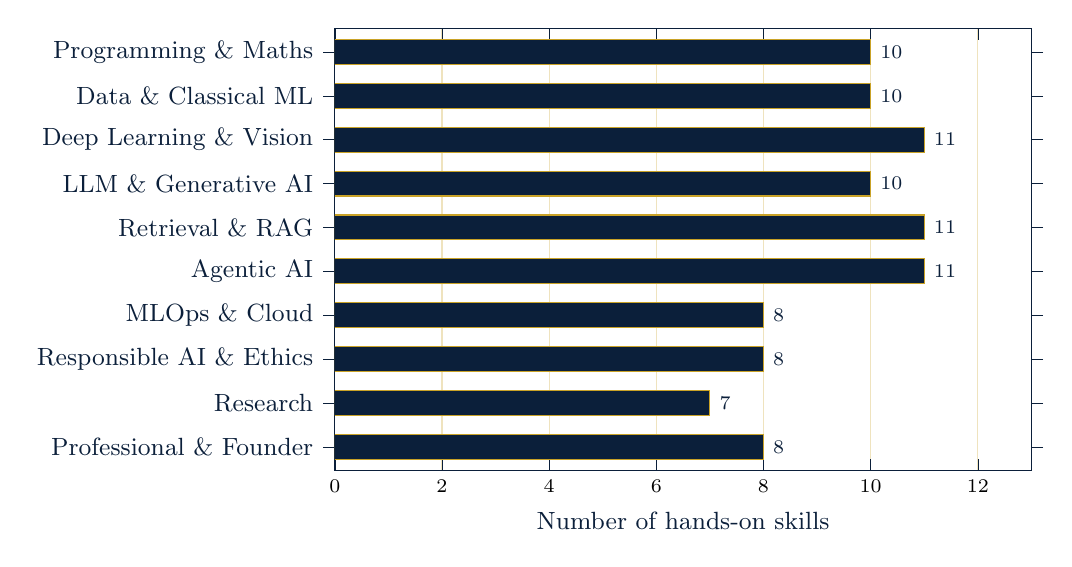
\begin{tikzpicture}
\begin{axis}[xbar,width=0.86\linewidth,height=7.2cm,bar width=9pt,xmin=0,xmax=13,
  symbolic y coords={Professional \& Founder,Research,Responsible AI \& Ethics,MLOps \& Cloud,Agentic AI,Retrieval \& RAG,LLM \& Generative AI,Deep Learning \& Vision,Data \& Classical ML,Programming \& Maths},
  ytick=data,y dir=normal,enlarge y limits=0.06,
  xlabel={Number of hands-on skills},xlabel style={font=\small,text=navy},
  yticklabel style={font=\small,text=navy},xticklabel style={font=\scriptsize},
  nodes near coords,nodes near coords style={font=\scriptsize\bfseries,text=navy},
  axis line style={navy},tick style={navy},major grid style={gold!30},xmajorgrids,
  every axis plot/.append style={fill=navy,draw=gold}]
\addplot[fill=navy,draw=gold] coordinates {(10,Programming \& Maths) (10,Data \& Classical ML) (11,Deep Learning \& Vision) (10,LLM \& Generative AI)
  (11,Retrieval \& RAG) (11,Agentic AI) (8,MLOps \& Cloud) (8,Responsible AI \& Ethics) (7,Research) (8,Professional \& Founder)};
\end{axis}
\end{tikzpicture}
\captionof{figure}{Hands-on skills per cluster: 94 skills in total, every one practised in a timed course hour.}
\end{center}

%% ======================= 4c. JOBS =======================
\newpage
\section{Jobs You Can Target After This Course}
Each role below lists what the job involves and which course projects give you evidence for it. Entry-level and junior roles are the realistic first target. Senior roles follow with experience.

\footnotesize
\rowcolors{2}{navy!5}{white}
\begin{tabularx}{\linewidth}{@{}L{3.3cm} Y L{4.2cm} L{1.5cm}@{}}
\rowcolor{navy}\color{gold}\sffamily\bfseries Job role & \color{gold}\sffamily\bfseries What you do on the job & \color{gold}\sffamily\bfseries Key skills from this course & \color{gold}\sffamily\bfseries Proof\\
AI Engineer & Build AI features into products using LLMs, RAG and agents & LLM APIs, RAG, FastAPI, evaluation & P3, P4, P5\\
Machine Learning Engineer & Train, tune and deploy ML models at scale & scikit-learn, PyTorch, MLflow, Docker & P1, P2, P6\\
LLM / GenAI Engineer & Fine-tune, evaluate and serve language models & LoRA, HF Transformers, vLLM, evals & P3\\
Agentic AI Engineer & Design multi-agent systems that use tools safely & LangGraph, MCP, sandboxing, tracing & P5\\
RAG / Search Engineer & Build enterprise search and document Q\&A & Embeddings, vector DBs, re-ranking, RAGAS & P4\\
Forward Deployed Engineer & Ship AI solutions on-site with enterprise customers & End-to-end build, pitching, deployment & P4, P6\\
Data Scientist & Turn business data into models and decisions & EDA, boosting, SHAP, storytelling & P1\\
Computer Vision Engineer & Build image and video recognition systems & CNN/ViT, Grad-CAM, ONNX, quantisation & P2\\
MLOps Engineer & Automate training, deployment and monitoring & Docker, CI/CD, drift monitoring, registry & P6\\
AI Research Engineer & Turn research ideas into working, tested code & Paper reproduction, PyTorch, experiments & P3, P5\\
Applied Scientist (junior) & Design experiments and new models for products & Experiment design, evaluation, ablations & P3, P4\\
Responsible AI Analyst & Audit models for bias, safety and compliance & Fairlearn, red-teaming, AI regulation & P6 audit\\
AI Product Engineer & Build full-stack AI apps that users love & FastAPI, streaming UX, product thinking & P4, P6\\
AI Solutions Architect (junior) & Design AI systems for client problems & System design, cost and latency trade-offs & P4, P5, P6\\
AI Trainer / Educator & Teach and mentor AI teams in companies and colleges & All modules, communication & Demo Day\\
AI Start-up Founder & Turn a capstone into a product and company & MVP building, pitching, product thinking & P6\\
\end{tabularx}
\normalsize

\subsection*{Where these jobs are}
\begin{tabularx}{\linewidth}{@{}L{4.4cm} Y@{}}
\toprule
\sffamily\bfseries Employer type & \sffamily\bfseries Why this course fits\\
\midrule
Top AI labs \& big tech & Need deep LLM, evaluation and system-design skills (Sundays 3--6)\\
Global Capability Centres (Hyderabad, Pune, Bengaluru) & Hire AI, RAG and MLOps engineers in large numbers (Sundays 4--6)\\
AI start-ups (India, USA, Canada) & Want builders who ship end-to-end and work fast (all BUILD hours)\\
IT services \& consulting & Need GenAI and agent engineers for client projects (Sundays 3--5)\\
Product companies (fintech, health, agri, ed-tech) & Need applied ML and vision skills (Sundays 1--2)\\
Universities \& research labs & Need research engineers who can reproduce and extend papers (Hrs 14, 23--24)\\
\bottomrule
\end{tabularx}

\vspace{6pt}
\begin{center}
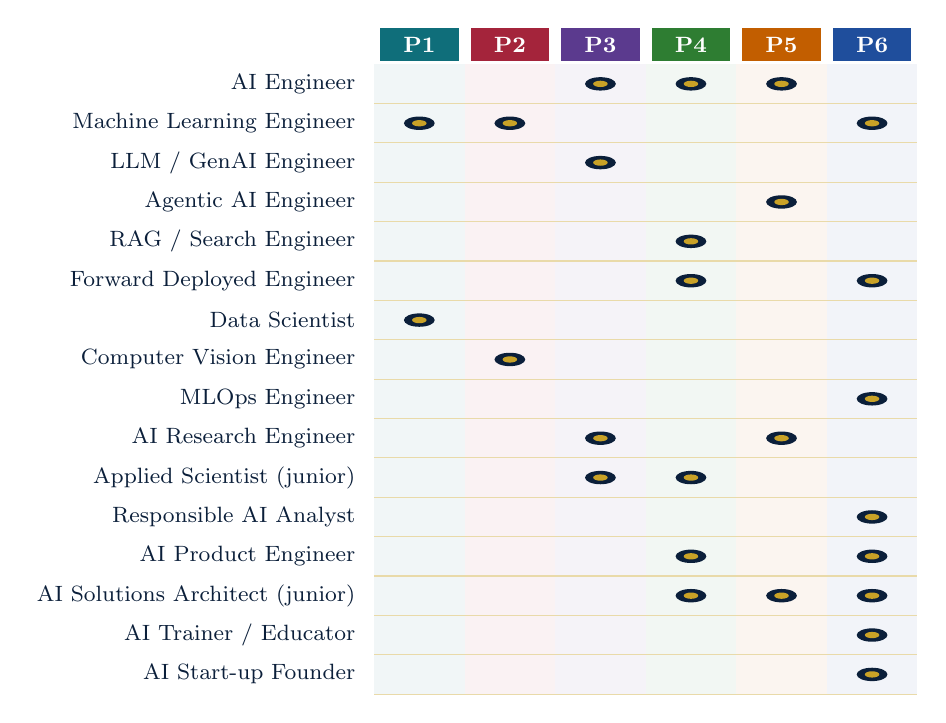
\begin{tikzpicture}[x=1.15cm,y=0.5cm,font=\footnotesize]
  \foreach \c/\p/\col in {1/P1/sunA,2/P2/sunB,3/P3/sunC,4/P4/sunD,5/P5/sunE,6/P6/sunF}{
    \node[fill=\col,text=white,minimum width=1.0cm,font=\footnotesize\bfseries] at (\c,1) {\p};
    \fill[\col!6] (\c-0.5,0.5) rectangle (\c+0.5,-15.5);
  }
  \foreach \r/\role/\ps in {0/AI Engineer/{3,4,5},1/Machine Learning Engineer/{1,2,6},2/{LLM / GenAI Engineer}/{3},3/Agentic AI Engineer/{5},
     4/{RAG / Search Engineer}/{4},5/Forward Deployed Engineer/{4,6},6/Data Scientist/{1},7/Computer Vision Engineer/{2},
     8/MLOps Engineer/{6},9/AI Research Engineer/{3,5},10/Applied Scientist (junior)/{3,4},11/Responsible AI Analyst/{6},
     12/AI Product Engineer/{4,6},13/AI Solutions Architect (junior)/{4,5,6},14/{AI Trainer / Educator}/{6},15/AI Start-up Founder/{6}}{
    \node[anchor=east,text=navy] at (0.4,-\r) {\role};
    \draw[gold!40] (0.5,-\r-0.5) -- (6.5,-\r-0.5);
    \foreach \c in \ps { \fill[navy] (\c,-\r) circle (0.17); \fill[gold] (\c,-\r) circle (0.08); }
  }
\end{tikzpicture}
\captionof{figure}{Job-role to project map. A dot means that project is direct portfolio evidence for the role.}
\end{center}

%% ======================= 5. ASSESSMENT =======================
\section{Assessment \& Certification}\label{sec:assess}
\begin{tabularx}{\linewidth}{@{}Y r@{}}
\toprule
\sffamily\bfseries Component & \sffamily\bfseries Weight\\
\midrule
Weekly project deliverables P1--P5 submitted on GitHub by 18:00 (code quality, results, README) & 50\%\\
Capstone P6 (deployment, audit, Demo Day pitch) & 30\%\\
Hour-5 mentor reviews and peer code reviews & 10\%\\
Career Lab mock interview & 10\%\\
\bottomrule
\end{tabularx}
\begin{itemize}
  \item \textbf{Certified} at 60\% overall and 5 of 6 Sundays attended. \textbf{Distinction} at 85\%.
  \item Every certificate carries a verification ID and the learner's GitHub portfolio link.
\end{itemize}

%% ======================= 6. ROADMAP 2026-2035 =======================
\newpage
\section{AI Skill Roadmap 2026 -- 2035}
This roadmap shows where AI skills are likely to move over the next decade, and which parts of this course carry forward. Later periods are projections from current research trends, not certainties. Each wave builds on the skills before it.

\vspace{4pt}
\begin{center}

\begin{tikzpicture}[x=1cm,y=1cm]
  \draw[gold,line width=2pt] (0,0) -- (17,0);
  \foreach \x/\y/\c in {1.4/2026--27/sunA,4.8/2028--29/sunB,8.2/2030--31/sunC,11.6/2032--33/sunD,15.0/2034--35/sunE}{
    \fill[\c] (\x,0) circle (0.22);
    \node[font=\sffamily\bfseries\small,text=navy] at (\x,0.6) {\y};
  }
\end{tikzpicture}
\captionof{figure}{AI skill waves, 2026--2035. Later waves are projections from current research trends.}
\end{center}

\small
\rowcolors{2}{goldlight!50}{white}
\begin{tabularx}{\linewidth}{@{}L{1.7cm} L{3.3cm} Y L{3.6cm}@{}}
\rowcolor{navy}\color{gold}\sffamily\bfseries Period & \color{gold}\sffamily\bfseries Skill wave & \color{gold}\sffamily\bfseries Skills to master & \color{gold}\sffamily\bfseries Roles in demand\\
\textbf{2026--27} & Agentic AI \& LLM engineering \newline {\color{sunA}\scriptsize\bfseries Covered in this course} &
  Agents and MCP tools, RAG, LoRA fine-tuning, LLM and agent evaluation, inference cost control, AI security basics &
  AI Engineer, Agent Engineer, Forward Deployed Engineer, LLM Ops Engineer\\
\textbf{2028--29} & Multimodal \& embodied AI &
  Vision-language-action models, real-time speech agents, video understanding, robotics foundation models, simulation-to-real transfer &
  Multimodal ML Engineer, Robotics AI Engineer, Voice AI Engineer\\
\textbf{2030--31} & AI for science \& autonomous research &
  AI-scientist agents that design and run experiments, scientific simulation, protein and materials modelling, causal inference &
  AI Research Scientist, Computational Scientist, AI-for-Science Lead\\
\textbf{2032--33} & Efficient, edge \& new-compute AI &
  On-device models, energy-aware training, neuromorphic and quantum-classical hybrid methods, privacy-preserving and federated learning &
  Edge AI Engineer, Green AI Engineer, Quantum ML Researcher\\
\textbf{2034--35} & Trustworthy advanced AI \& governance &
  Interpretability, alignment and safety evaluation, AI auditing and certification, global AI regulation, human--AI team design &
  AI Safety Researcher, AI Auditor, Chief AI Officer, AI Policy Advisor\\
\end{tabularx}
\normalsize

\begin{goldnote}\textbf{Skills that last the whole decade:} mathematics for ML, clean code, experiment design, evaluation discipline, reading research papers, ethics and clear communication. This course trains each of them every Sunday.\end{goldnote}

%% ======================= 7. CAREER =======================
\section{Career Readiness: Top AI Companies \& AI Start-ups}

\subsection*{What hiring teams test, and where this course trains it}
\small
\rowcolors{2}{navy!5}{white}
\begin{tabularx}{\linewidth}{@{}L{4.6cm} Y L{2.6cm}@{}}
\rowcolor{navy}\color{gold}\sffamily\bfseries Interview area & \color{gold}\sffamily\bfseries What they look for & \color{gold}\sffamily\bfseries Trained in\\
ML fundamentals & Bias--variance, metrics, leakage, validation design & Hrs 1--5\\
Deep learning depth & Backprop, optimisation, architecture trade-offs & Hrs 6--12\\
LLM \& agent depth & Attention, fine-tuning, RAG, agent failure modes, evaluation & Hrs 11--25\\
ML system design & Design an end-to-end system with latency, cost and monitoring & Hrs 15, 19, 26, 28\\
Coding \& debugging & Clean Python, tests, reading unfamiliar code & Every BUILD hour\\
Responsible AI & Fairness, safety, privacy and regulation awareness & Hr 27\\
Start-up readiness & Ship fast, talk to users, pitch clearly & Hrs 29--30\\
\end{tabularx}
\normalsize

\subsection*{Target career tracks}
\begin{itemize}
  \item \textbf{Top AI and big-tech companies:} AI/ML Engineer, Applied Scientist, LLM Engineer, Forward Deployed Engineer.
  \item \textbf{AI start-ups:} founding AI engineer, agent engineer, full-stack AI product engineer.
  \item \textbf{Research path:} research assistant, Ph.D./postdoc pathway through AlgoProfessor research mentoring.
  \item \textbf{Founder path:} turn the capstone into a minimum viable product, with a start-up clinic in Hour 30.
\end{itemize}

\subsection*{90-day plan after the course}
\begin{tabularx}{\linewidth}{@{}L{2.4cm} Y@{}}
\toprule
\sffamily\bfseries Days 1--30 & Polish all 6 repositories. Write one technical blog post per project. Solve 40 coding problems.\\
\sffamily\bfseries Days 31--60 & Extend the capstone with real users. Enter one Kaggle or Hugging Face competition. Contribute to one open-source AI library.\\
\sffamily\bfseries Days 61--90 & Apply to 30+ targeted roles, ask for referrals, run 5 more mock interviews, take the AlgoProfessor Level 2 track.\\
\bottomrule
\end{tabularx}

\begin{navynote}
\textbf{\color{gold}An honest note on outcomes.} Thirty hours gives you a strong, portfolio-backed start: six shipped projects and the vocabulary top teams use. Offers from top AI companies and funded start-ups also depend on sustained practice, coding interviews, and work you keep building after the course. The 90-day plan is there for that. AlgoProfessor gives mentoring and referrals where it can, but does not guarantee placement.
\end{navynote}


%% ======================= GITHUB SUBMISSION POLICY =======================
\newpage
\section{GitHub Submission Policy: 18:00 Every Sunday}
\begin{navynote}
\textbf{\color{gold}Rule.} Every learner submits that Sunday's project on GitHub \textbf{by 18:00 local time on the same Sunday} (IST in Hyderabad and Shirdi; local time in the USA and Canada). The teaching day ends at 15:00. The three hours until 18:00 are for clean-up, documentation and pushing. Work not submitted correctly by 18:00 is graded as late.
\end{navynote}

\subsection*{1. One portfolio repository per learner}
Create one \textbf{public} repository on day one and use it for all six Sundays. Name it exactly:
\begin{center}\texttt{\large algoprofessor-ai-scientist-<campus>-<batch>-<learnerID>}\end{center}
Example: \texttt{algoprofessor-ai-scientist-hyd-b01-AP2601023}. Campus codes: \texttt{hyd} Hyderabad, \texttt{sdi} Shirdi, \texttt{usa} USA, \texttt{can} Canada.

\subsection*{2. Required folder structure}
\begin{minipage}[t]{0.47\linewidth}\vspace{0pt}
\begin{tcolorbox}[colback=navy,colframe=gold,boxrule=0.7pt,arc=2pt,coltext=white,fontupper=\small\ttfamily,left=6pt]
algoprofessor-ai-scientist-.../\\
\hspace*{1em}README.md \hfill {\color{gold}portfolio index}\\
\hspace*{1em}LICENSE \hfill {\color{gold}MIT or Apache-2.0}\\
\hspace*{1em}.gitignore\\
\hspace*{1em}P1-churn-intelligence/\\
\hspace*{1em}P2-leafdoctor/\\
\hspace*{1em}P3-minillm/\\
\hspace*{1em}P4-policygpt/\\
\hspace*{1em}P5-scholaragent/\\
\hspace*{1em}P6-capstone/
\end{tcolorbox}
\end{minipage}\hfill
\begin{minipage}[t]{0.49\linewidth}\vspace{0pt}
\begin{tcolorbox}[colback=goldlight,colframe=gold,boxrule=0.7pt,arc=2pt,fontupper=\small\ttfamily,left=6pt]
P\textit{n}-project-name/\\
\hspace*{1em}README.md \hfill {\color{navylight}project report}\\
\hspace*{1em}requirements.txt\\
\hspace*{1em}notebooks/ \hfill {\color{navylight}exploration}\\
\hspace*{1em}src/ \hfill {\color{navylight}clean, reusable code}\\
\hspace*{1em}results/ \hfill {\color{navylight}metrics, plots}\\
\hspace*{1em}docs/ \hfill {\color{navylight}model card, slides}\\
\hspace*{1em}data/README.md \hfill {\color{navylight}links only}
\end{tcolorbox}
\end{minipage}

\subsection*{3. Project README must contain}
\small
\rowcolors{2}{navy!5}{white}
\begin{tabularx}{\linewidth}{@{}L{4.0cm} Y@{}}
\rowcolor{navy}\color{gold}\bfseries Section & \color{gold}\bfseries What to write\\
Problem statement & The question you solved, who it helps, and the success metric\\
Dataset & Name, source link, licence, size, and how to download it\\
Method & Model and pipeline, with one architecture diagram\\
Results & Metrics table, key plots, and comparison with the baseline\\
How to run & Exact commands to install and reproduce the results\\
Limitations \& ethics & Where it fails, bias checks, and risks\\
AI-assistant use & Which AI tools you used and for which parts (honest disclosure)\\
Author & Name, learner ID, campus, batch, and Sunday number\\
\end{tabularx}
\normalsize

\subsection*{4. Step-by-step submission (every Sunday)}
\begin{enumerate}[leftmargin=1.6em,itemsep=2pt]
  \item \textbf{Commit as you work.} Make at least 3 meaningful commits during the BUILD hours, e.g.\ \texttt{feat(P2): add Grad-CAM visualisation}. One large commit at 17:59 is not accepted as evidence of the day's work.
  \item \textbf{Clean up.} Run the notebook top to bottom, remove dead code, update \texttt{requirements.txt} and the README.
  \item \textbf{Push} to the \texttt{main} branch: \texttt{git push origin main}.
  \item \textbf{Tag the release:} \texttt{git tag -a sunday-}\textit{n}\texttt{ -m "Sunday }\textit{n}\texttt{ submission"} then \texttt{git push origin sunday-}\textit{n}.
  \item \textbf{Create a GitHub Release} from the tag, attaching slides or the report PDF if any.
  \item \textbf{Submit} the release link and the commit hash on the AlgoProfessor submission form shared in class, before 18:00.
\end{enumerate}

\subsection*{5. Never commit}
\begin{goldnote}
API keys, passwords or tokens (use a \texttt{.env} file and list it in \texttt{.gitignore}) $\cdot$ raw datasets or files larger than 50 MB (put download links in \texttt{data/README.md}, or use Git LFS) $\cdot$ personal data of real people $\cdot$ copied code without credit. A leaked key must be revoked at once and reported to your mentor.
\end{goldnote}

\subsection*{6. Late and missing submissions}
\begin{tabularx}{\linewidth}{@{}L{4.2cm} Y@{}}
\toprule
\bfseries Submitted & \bfseries Effect on that project's marks\\
\midrule
By 18:00 Sunday & Full marks available\\
18:01 -- 23:59 Sunday & 10\% deduction\\
Monday -- Wednesday & 25\% deduction\\
After Wednesday or not tagged & Not graded. Counts against certification.\\
\bottomrule
\end{tabularx}
Mentors review each tagged release before the next Sunday and leave feedback as GitHub Issues in your repository.

%% ======================= 8. CAMPUSES =======================
\section{Offline Campuses \& Enrolment}
\begin{tabularx}{\linewidth}{@{}L{2.8cm} L{3.2cm} L{2.4cm} Y@{}}
\toprule
\sffamily\bfseries Campus & \sffamily\bfseries Batch day \& time & \sffamily\bfseries Fee & \sffamily\bfseries Notes\\
\midrule
Hyderabad, India & Sundays, 09:00--15:00 IST & INR 50,000 & Flagship campus. AlgoProfessor AI R\&D Solutions.\\
Shirdi, India & Sundays, 09:00--15:00 IST & INR 50,000 & Regional campus for learners in Maharashtra.\\
USA & Sundays, 09:00--15:00 local & US\$ 1,000 & City and venue announced per batch.\\
Canada & Sundays, 09:00--15:00 local & US\$ 1,000 & City and venue announced per batch.\\
\bottomrule
\end{tabularx}

\vspace{6pt}
\begin{navynote}
\textbf{\color{gold}Enrolment \& partnership enquiries}\\[3pt]
Applications: cto@algoprofessor.com \quad$\cdot$\quad Director: ceo@algoprofessor.com\\
Web: www.algoprofessor.com\\[4pt]
{\color{goldlight}Dr S Satyanarayana Ph.D., PDF(AI), FARSC --- Founder \& CEO, AlgoProfessor $\cdot$ Creator of AlgoLang}
\end{navynote}


%% ======================= CERTIFICATE FORMAT =======================
\newpage
\section{Certificate Format}
The certificate below is issued to every learner who meets the certification rules in Section~\ref{sec:assess}. Fields in angle brackets are filled per learner.

\begin{tabularx}{\linewidth}{@{}L{4.2cm} Y@{}}
\toprule
\bfseries Item & \bfseries Format\\
\midrule
Title & Certificate of Completion --- AlgoProfessor AI Scientist, Hands-On (Level 1)\\
Result levels & \emph{Certified} (60\% or more) or \emph{Certified with Distinction} (85\% or more)\\
Certificate number & \texttt{AP-AIS-L1-<YYYY>-<campus>-<serial>}, e.g.\ \texttt{AP-AIS-L1-2026-HYD-0042}\\
Signatories & Course Director and Campus Programme Lead\\
Verification & QR code and certificate number, checkable on the AlgoProfessor website\\
Portfolio link & The learner's GitHub repository, printed on the certificate\\
Issue & Printed copy at Demo Day; digital PDF within 7 days\\
Paper & A4 landscape, 300 gsm ivory card, navy and gold print\\
\bottomrule
\end{tabularx}

\newgeometry{margin=0.6cm}
\begin{landscape}
\thispagestyle{empty}
\centering

\begin{tikzpicture}
  \coordinate (C) at (0,0);
  %% outer frame
  \path (-13.85,9.6) rectangle (13.85,-9.6);
  \draw[navy,line width=6pt] ($(-13.85,9.6)+(0.2,-0.2)$) rectangle ($(13.85,-9.6)+(-0.2,0.2)$);
  \draw[gold,line width=1.5pt] ($(-13.85,9.6)+(0.55,-0.55)$) rectangle ($(13.85,-9.6)+(-0.55,0.55)$);
  \draw[gold,line width=0.4pt] ($(-13.85,9.6)+(0.75,-0.75)$) rectangle ($(13.85,-9.6)+(-0.75,0.75)$);
  %% tricolour accent strips
  \fill[saffron] ($(-13.85,9.6)+(0.75,-0.75)$) rectangle ($(13.85,9.6)+(-0.75,-1.05)$);
  \fill[indgreen] ($(-13.85,-9.6)+(0.75,0.75)$) rectangle ($(13.85,-9.6)+(-0.75,1.05)$);
  %% corner ornaments
  \node[draw=gold,fill=goldlight,diamond,minimum size=0.55cm] at ($(-13.85,9.6)+(1.5,-1.8)$) {};
  \node[draw=gold,fill=goldlight,diamond,minimum size=0.55cm] at ($(13.85,9.6)+(-1.5,-1.8)$) {};
  \node[draw=gold,fill=goldlight,diamond,minimum size=0.55cm] at ($(-13.85,-9.6)+(1.5,1.8)$) {};
  \node[draw=gold,fill=goldlight,diamond,minimum size=0.55cm] at ($(13.85,-9.6)+(-1.5,1.8)$) {};
  %% header
  \node[text=navy,font=\bfseries\fontsize{26}{28}\selectfont] at ($(C)+(0,7.0)$) {AlgoProfessor};
  \node[text=navylight,font=\small] at ($(C)+(0,6.2)$) {AI R\&D Solutions $\cdot$ Hyderabad, India $\cdot$ www.algoprofessor.com};
  \draw[gold,line width=1pt] ($(C)+(-5,5.75)$) -- ($(C)+(5,5.75)$);
  \node[text=gold!85!black,font=\bfseries\scshape\fontsize{30}{34}\selectfont] at ($(C)+(0,4.75)$) {Certificate of Completion};
  \node[text=ink,font=\large\itshape] at ($(C)+(0,3.55)$) {This is to certify that};
  \node[text=navy,font=\bfseries\fontsize{28}{32}\selectfont] at ($(C)+(0,2.4)$) {<Learner Full Name>};
  \draw[gold,line width=0.8pt] ($(C)+(-7,1.75)$) -- ($(C)+(7,1.75)$);
  \node[text=ink,font=\large,align=center,text width=21cm] at ($(C)+(0,0.45)$)
    {has successfully completed the 30-hour \textbf{AlgoProfessor AI Scientist --- Hands-On (Level 1)} programme,\\
     Sunday Edition, comprising 12 hours of hands-on teaching and 18 hours of real-time project work,\\
     and has shipped six portfolio projects on GitHub, including one capstone deployed to production.};
  %% details row
  \foreach \x/\h/\v in {-9.6/Campus/<Hyderabad | Shirdi | USA | Canada>,-3.2/Batch \& Dates/<B01 \;$\cdot$\; DD Mon -- DD Mon YYYY>,
                       3.2/Result/<Certified | Distinction>,9.6/Learner ID/<AP26xxxxx>}{
    \node[text=gold!85!black,font=\footnotesize\bfseries\scshape] at ($(C)+(\x,-1.55)$) {\h};
    \node[text=navy,font=\small] at ($(C)+(\x,-2.1)$) {\v};
  }
  \node[text=navylight,font=\small] at ($(C)+(0,-3.0)$) {GitHub portfolio: \texttt{github.com/<username>/algoprofessor-ai-scientist-<campus>-<batch>-<learnerID>}};
  %% seal
  \node[circle,fill=navy,draw=gold,line width=2pt,minimum size=3.1cm] (seal) at ($(C)+(0,-5.35)$) {};
  \node[circle,draw=gold,line width=0.6pt,minimum size=2.6cm] at (seal) {};
  \node[text=gold,font=\bfseries\footnotesize,align=center] at (seal) {AI SCIENTIST\\[-1pt]{\scriptsize HANDS-ON}\\[-1pt]{\large\bfseries L1}\\[-1pt]{\scriptsize 2026}};
  %% signatures
  \draw[navy,line width=0.6pt] ($(C)+(-11.0,-5.3)$) -- ($(C)+(-4.0,-5.3)$);
  \node[text=navy,font=\small\bfseries,align=center] at ($(C)+(-7.5,-5.85)$) {Dr S Satyanarayana Ph.D., PDF(AI), FARSC};
  \node[text=navylight,font=\footnotesize,align=center] at ($(C)+(-7.5,-6.35)$) {Course Director $\cdot$ Founder \& CEO, AlgoProfessor};
  \draw[navy,line width=0.6pt] ($(C)+(4.0,-5.3)$) -- ($(C)+(11.0,-5.3)$);
  \node[text=navy,font=\small\bfseries,align=center] at ($(C)+(7.5,-5.85)$) {<Campus Programme Lead>};
  \node[text=navylight,font=\footnotesize,align=center] at ($(C)+(7.5,-6.35)$) {Lead Mentor, <Campus>};
  %% verification
  \node[draw=navy,line width=0.6pt,minimum size=1.7cm,text=navylight,font=\scriptsize,align=center] at ($(C)+(11.6,-3.0)$) {QR\\verify};
  \node[text=navylight,font=\scriptsize,anchor=west] at ($(C)+(-12.4,-7.45)$) {Certificate No.: AP-AIS-L1-<YYYY>-<campus>-<serial>};
  \node[text=navylight,font=\scriptsize,anchor=east] at ($(C)+(12.4,-7.45)$) {Verify at www.algoprofessor.com/verify \;$\cdot$\; Issued: <DD Month YYYY>};
\end{tikzpicture}
\end{landscape}
\restoregeometry

\end{document}
